%! Author = Len Washington III
%! Date = 10/10/2023

% Preamble
\documentclass[12pt]{report}

% Packages
\usepackage[15]{cs430lecture}
\usepackage{algpseudocode}

% Document
\begin{document}

%<*Lecture-Activity-15>
\newcommand{\examplesep}{\mbox{ }\mbox{ }\mbox{ }\mbox{ }\mbox{ }\mbox{ }}
\section{Opening Questions}\label{sec:opening-questions-15}
\begin{enumerate}[label=\arabic*.]
    \item Why are optimal solutions to sub-problems stored in dynamic programming solutions?\answer{\ You only have to store the optimal answer for the subproblem because optimal substructure says that the overlapping subproblems only needs to know the optimal solution, not any other solution.}
\end{enumerate}

Constructing the answer for the Optimal Matrix Chain Multiplication (optimal parenthesization) from the dynamic programming table. See the solution to the example problem
\begin{table}[H]
    \centering
    \begin{threeparttable}
		\label{tab:optimal-matrix-chain-programming}
		\begin{tabular}{cccccc}
			$A_{1}$ & $A_{2}$ & $A_{3}$ & $A_{4}$ & $A_{5}$ & $A_{6}$\\
            $30\times35$ & $35\times15$ & $15\times5$ & $5\times10$ & $10\times20$ & $20\times25$
		\end{tabular}
	\end{threeparttable}
\end{table}

\begin{table}[H]
    \centering
    \begin{threeparttable}
		\label{tab:optimal-matrix-chain-images}
		\begin{tabular}{|l|l|}
			\toprule
			\begin{minipage}{0.45\textwidth}
				\begin{figure}[H]
					\centering
					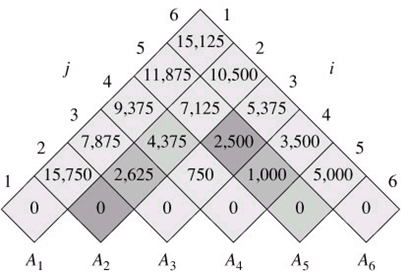
\includegraphics[width=\textwidth]{15.1}
					\label{fig:optimal-matrix-chain-p-table}
				\end{figure} P table
            \end{minipage} &
			\begin{minipage}{0.45\textwidth}
				\begin{figure}[H]
					\centering
					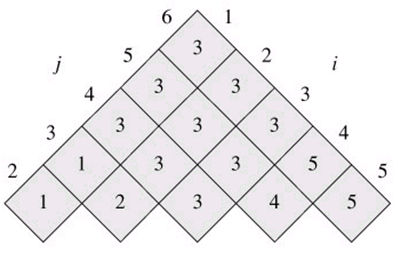
\includegraphics[width=\textwidth]{15.2}
					\label{fig:optimal-matrix-chain-root-table}
				\end{figure}Root table
            \end{minipage}\\
			\bottomrule
		\end{tabular}
	\end{threeparttable}
\end{table}
\begin{enumerate}[label=\arabic*.,start=2]
    \item Write the optimal parenthesization.\answer{\begin{equation*}
    \begin{aligned}
    	A_{1} & A_{2} & A_{3} & A_{4} & A_{5} & A_{6}\\
    	( A_{1} & A_{2} & A_{3} ) & ( A_{4} & A_{5} & A_{6} )\\
    	( (A_{1}) & (A_{2} & A_{3}) ) & ( A_{4} & A_{5} & A_{6} )\\
    	( (A_{1}) & (A_{2} & A_{3}) ) & ( (A_{4} & A_{5}) & A_{6} )\\
    \end{aligned}
    \end{equation*}}
	\item Write pseudocode to use the root table to print the optimal parenthesization. Then write pseudocode to use the root table to actually perform the multiplications in the optimal parenthesization.\answer{\begin{algorithm}[H]
		\caption{Print Optimal Parenthesization for Matrix Chain Multiplication}\label{alg:print-opt-parens}
		\begin{algorithmic}[1]
		\Function{PrintOptParens}{$root$, $from$, $to$}\Comment{Initial Call: \Call{PrintOptParens}{$root$, $1$, $n$}}
			\If{$from == to$}
				\State \Call{Print}{"$A_{from}$"}
			\Else
				\State \Call{Print}{"$($"}
				\State \Call{PrintOptParens}{$root$, $from$, $root$[$from$,$to$]} \Comment{The $root[from,to]$ states the index that was extracted from the root table.}
				\State \Call{Print}{"$\times$"}
				\State \Call{PrintOptParens}{$root$, $root$[$from$,$to$]+1, $to$}
				\State \Call{Print}{"$)$"}
			\EndIf
		\EndFunction
		\end{algorithmic}
	\end{algorithm} Assume we have a function \Call{MultMatrix}{$x$, $y$} that multiplies 2 matrices and returns the results(given correct dimensions.) \begin{algorithm}[H]
		\caption{Multiply Optimal Parenthesization for Matrix Chain Multiplication}\label{alg:mult-opt-parens}
		\begin{algorithmic}[1]
		\Function{MultOptParens}{$root$, $from$, $to$}\Comment{Initial Call: \Call{MultOptParens}{$root$, $1$, $n$}}
			\If{$from == to$}
				\State \Return $A_{from}$
			\Else
				\State $a \gets $ \Call{MultOptParens}{$root$, $from$, $root$[$from$,$to$]}
				\State $b \gets $ \Call{MultOptParens}{$root$, $root$[$from$,$to$] + 1, $to$}
				\State \Return \Call{MultMatrix}{$a$, $b$}
			\EndIf
		\EndFunction
		\end{algorithmic}
	\end{algorithm}}
\end{enumerate}

\section{Longest Common Subsequence}\label{sec:longest-common-subsequence}
Example: $X[1\dots m] \examplesep Y[1\dots n]$

$X=ABCBDAB \examplesep Y=BDCABA$

Length of LCS = 4 $BCBA$ or $BCAB$

\begin{enumerate}[label=\arabic*.]
    \item The brute force (try all possibilities) approach would be to find all subsequences of one input, see if each exists in other input. How many are there? \answer{Assume $m < n$. You would have the choices: $\frac{2}{1}$ $\frac{2}{2}$ $\frac{2}{3}$ $\frac{2}{4} \dots$ $\frac{2}{m-2}$ $\frac{2}{m-1}$ $\frac{2}{m}$, where the two represents that there are 2 choices for each position, yes or no, including all no's representing the empty set. This means there $2^{m}$ possible subsequences, again assuming that $m$ is smaller than $n$. For each generated subsequence, you have to check if it's in $Y$, which would take $O(n)$ for each check. The total runtime for brute force is $O(n2^{m})$.}
	\item Step 1: Generically define the structure of the optimal solution to the Longest Common Subsequence problem. The longest common sequence of sequence $X[1\dots m]$ and sequence $Y[1\dots n]$ is: \answer{\begin{figure}[H]
	   \centering
	   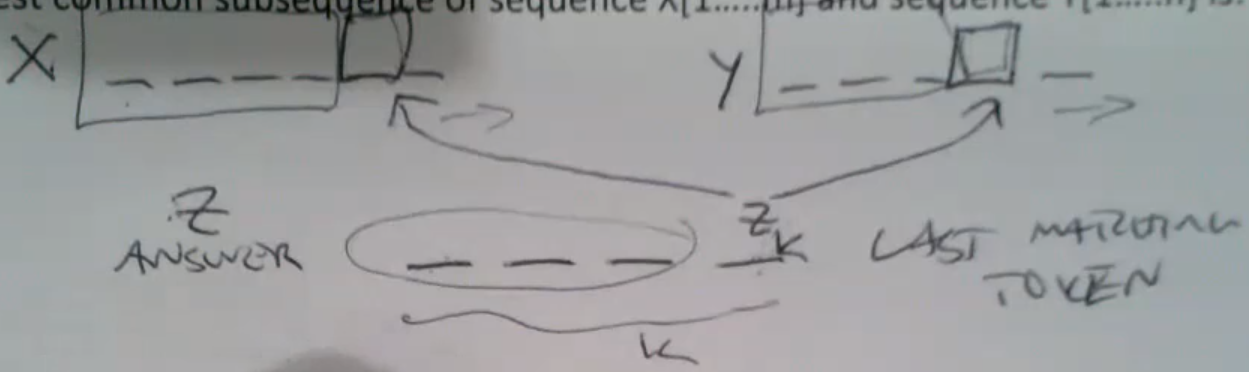
\includegraphics[width=\textwidth]{15.3}
	\end{figure}
		\begin{algorithm}[H]
		\caption{Basic pseudocode for Longest Common Sequence}\label{alg:longest-common-sequence}
		\begin{algorithmic}[1]
		\Function{LongestCommonSequence}{$x$, $m$, $y$, $n$}
			\If{$x[m] == y[n]$}\Comment{Use it}
				\State Add 1 to the answer for the subproblem $x[1\dots(m-1)]$,$y[1\dots(n-1)]$
			\Else\Comment{}
				\State Max$\left\{ \begin{array}{l}
					\mbox{Answer for } x[1\dots m], y[1\dots(n-1)]\\
					\mbox{Answer for } x[1\dots(m-1)], y[1\dots n]
				\end{array} \right.$
			\EndIf
		\EndFunction
		\end{algorithmic}
	\end{algorithm}}
	\item\label{prb:15-3} Step 2: Recursively define the optimal solution. Assume $C(i,j)$ is the optimal answer for up to position $i$ in $X$ and position $j$ in $Y$. Make sure you include the base case. \answer{\begin{equation*}
	\begin{aligned}
		C(i,j) = \left\{ \begin{array}{ll}
			C(i-1,j-1) & \mbox{ if } x[i] == y[j]\\
			\max \left\{ \begin{array}{l}
					C(i-1,j)\\
					C(i,j-1)
				\end{array} \right. & \mbox{ if } x[i] \neq y[j]
		\end{array} \right.
	\end{aligned}
	\end{equation*} Base Cases: \begin{itemize}
		\item $i == 0$
		\begin{itemize}
			\item $C(0,j) = 0$
			\item $C(i,0) = 0$
			\item $C(0,0) = 0$
		\end{itemize}
	\end{itemize}}
	\item Use proof by contradiction to show that Longest Common Subsequence problem has optimal substructure, i.e.\ the optimal answer to problem must contain optimal answers to sub-problems. \answer{Assume $z[1\dots k]$ is optimal for $x[1\dots i]$ and $y[1\dots j]$. If $z[k]=x[i]=y[j]$, then we have a subproblem $z[1\dots (k-1)]$ that must be optimal for $x[1\dots (i-1)]$ $y[1\dots (j-1)]$. The contradiction is that if someone said some sequence $w$ with length $k$ (or more) is optimal for $x[1\dots(i-1)]$, $y[1\dots(j-1)]$, which is longer than $z$, then you could add on the end of $w$ the characters that we know matches $(x[i]=y[j])$, then we would get a solution larger than $k$ for this problem. But that's impossible because we assumed $z[1\dots k]$ is the longest possible solution.}
	\item Step 3: Compute solution using a table bottom up for the Longest Common Subsequence problem. Use your answer to question \hyperref[prb:15-3]{3} above. Note the overlapping sub-problems as you go. \answer{\begin{table}[H]
	    \centering
	    \begin{threeparttable}
			\begin{tabular}{cc|c|cccccc}
										& 		& 		& \multicolumn{6}{c}{$Y$}\\
									$C$ &		&		&	$B$						&	$D$						& $C$						&	$A$							& $B$						& $A$\\
									\midrule
										&		& 0 	&  0						&  0						& 	0						&  0							& 0 						& 0\\
									\midrule
				\multirow{7}{*}{X}  	& $A$ 	& 0 	& $\rightarrow\downarrow0$	& $\rightarrow\downarrow0$	& $\rightarrow\downarrow0$	& $\searrow$1					& $\rightarrow$1			& $\searrow1$ \\
										& $B$ 	& 0 	& $\searrow1$				& $\rightarrow1$			& $\rightarrow1$			& $\rightarrow\downarrow1$		& $\searrow2$				& $\rightarrow2$ \\
										& $C$ 	& 0 	& $\downarrow1$				& $\rightarrow\downarrow1$	& $\searrow2$				& $\rightarrow2$				& $\rightarrow\downarrow2$	& $\rightarrow\downarrow2$ \\
										& $B$ 	& 0 	& $\searrow1$				& $\rightarrow\downarrow1$	& $\downarrow2$				& $\rightarrow\downarrow2$		& $\searrow3$				& $\rightarrow3$\\
										& $D$ 	& 0 	& $\downarrow1$				& $\searrow2$				& $\rightarrow\downarrow2$	& $\rightarrow\downarrow2$		& $\downarrow3$				& $\rightarrow\downarrow3$\\
										& $A$ 	& 0 	& $\downarrow1$				& $\downarrow2$				& $\rightarrow\downarrow2$	& $\searrow3$					& $\rightarrow\downarrow3$	& $\searrow4$\\
										& $B$ 	& 0 	& $\searrow1$				& $\downarrow2$				& $\rightarrow\downarrow2$	& $\downarrow3$					& $\searrow4$				& $\rightarrow\downarrow4$ \\
			\end{tabular}
		\end{threeparttable}\label{tab:longest-common-subsequence-example}
	\end{table}}
	\item Step 4: Construct Optimal Solution\answer{\ Walking backwards and adding the character when there was a match, there are 3 answers. $BCBA$, $BDAB$, $BCAB$ all of length 4.}
\end{enumerate}

$X=ABCBDAB \examplesep Y=BDCABA$

\url{https://www.cs.usfca.edu/~galles/visualization/DPLCS.html}
%</Lecture-Activity-15>

\end{document}